% This is samplepaper.tex, a sample chapter demonstrating the
% LLNCS macro package for Springer Computer Science proceedings;
% Version 2.20 of 2017/10/04




\documentclass[runningheads]{llncs}

\setcounter{secnumdepth}{3}


\usepackage[english]{babel}
\usepackage{graphicx}
\usepackage{verbatim}
\usepackage{tabularx}
\usepackage{float}
\usepackage{graphicx}
\usepackage{biblatex}
\usepackage{hyperref}
\usepackage{setspace}
\usepackage[table,xcdraw]{xcolor}
\addbibresource{referencias.bib}

% Used for displaying a sample figure. If possible, figure files should
% be included in EPS format.
%
% If you use the hyperref package, please uncomment the following line
% to display URLs in blue roman font according to Springer's eBook style:
% \renewcommand\UrlFont{\color{blue}\rmfamily}

\begin{document}
%
\title{EchoNet-Dynamic: U-Net for Cardiac Image Segmentation}
%
%\titlerunning{Abbreviated paper title}
% If the paper title is too long for the running head, you can set
% an abbreviated paper title here
%
    
\author{Salvador Mendoza\inst{1}\orcidID{A01067783} \and
Karla Gonzalez\inst{1}\orcidID{A01541526} \and
Alfonso Pineda\inst{1}\orcidID{A01660394} \and
Mariana Rincón\inst{1}\orcidID{A01654973} \and
Álvaro Morán\inst{1}\orcidID{A01638034}}
%

% First names are abbreviated in the running head.
% If there are more than two authors, 'et al.' is used.
%
\institute{Instituo Tecnológico y de Estudios Superiores de Monterrey, Campus Guadalajara.}
%
\maketitle              % typeset the header of the contribution
%
\begin{abstract}
This research employs a U-Net model for left ventricle segmentation in echocardiogram images, comparing two training approaches: binary masks and landmarks. Utilizing the EchoNet-Dynamic dataset, we evaluate model performance using the Dice Score. The study aims to determine the effectiveness of these training methodologies, providing insights into optimal strategies for U-Net models in cardiac image segmentation.


\keywords{Echocardiogram \and Deep Learning \and Image segmentation \and Neural Networks \and U-net \and Masks \and Landmarks \and Dice Score.}
\end{abstract}
%
%
%
\section{Introduction}
The echocardiogram is an indispensable ultrasound tool for evaluating cardiac function and structural characteristics, playing a vital role in diagnosing various cardiac conditions. This project is conducted in collaboration with EXO, a leading Canadian AI corporation dedicated to revolutionizing medical imaging accessibility. EXO's innovative advancements in medical technology have significantly contributed to extending healthcare accessibility worldwide. Through our collaboration with them, we aim to harness cutting-edge expertise in artificial intelligence for medical imaging, leveraging their pivotal contributions to refine and advance heart diagnostics using state-of-the-art computational methods such as neuronal networks.

Therefore, our dedicated focus in this research project is on the application of machine learning techniques to analyze echocardiogram data, with a particular emphasis on the segmentation assessment of the left ventricle—a critical indicator of overall heart performance. To provide a visual context for our research focus, Fig. \ref{fig:lv} illustrates a representative echocardiogram displaying the left ventricle's details. It is important to mention that this image displayed is inverted compared to the usual orientation in the datasets we have worked with. Typically, we are accustomed to locating the left ventricle in the upper right corner of the images \cite{cita}.

\begin{figure}[H]
  \centering
  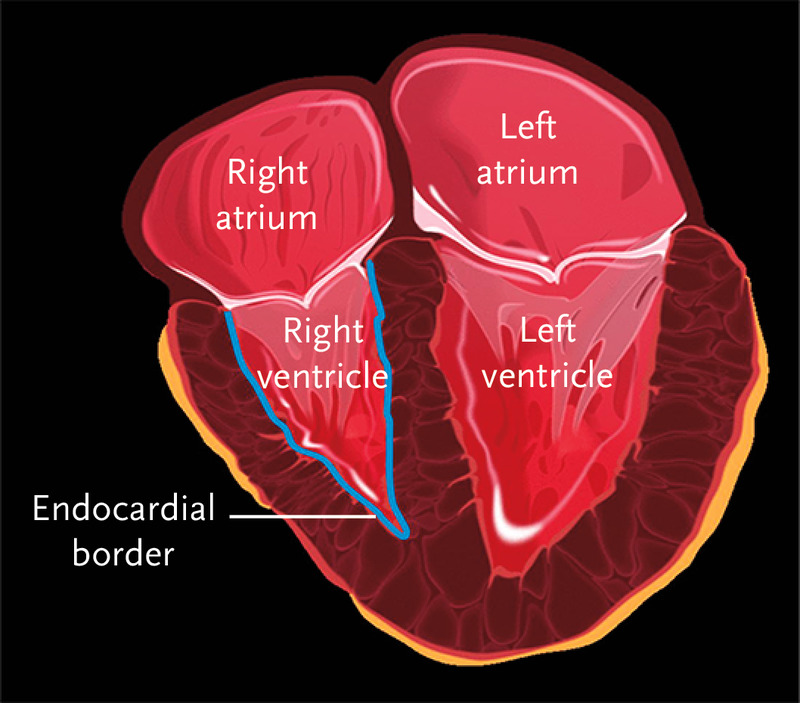
\includegraphics[width=0.5\textwidth]{lv.jpeg}
  \caption{Echocardiogram image with emphasis on the left ventricle}
  \label{fig:lv}
\end{figure}

This study aligns with a broader trend seeking to integrate deep learning methods into cardiac diagnostics, with a specific focus on comparing the efficacy of distinct image segmentation neural networks. We aim to determine which network demonstrates superior performance, both in achieving higher accuracy, which in this particular case would be the Dice Score, and in learning efficiency, particularly when trained with a limited number of images. Additionally, our research aims to identify and delineate the inherent advantages and disadvantages of each image segmentation network type. 

Current advancements in cardiac diagnostics have spurred the exploration of innovative methodologies, notably in the integration of machine learning for refined echocardiographic analysis. The work by Ali et al. \cite{a} represents a pioneering stride in this domain, proposing an image segmentation hybrid network, ResU, merging ResNet and U-Net architectures. This paper framework demonstrates substantial progress in accurate left ventricular segmentation within echocardiograms. Leveraging their innovative approach, our study aims to contribute to ongoing debates by delving into a comparative analysis of neural networks for echocardiogram analysis. Our exploration seeks to shed empirical insights on optimal computational models for precise ventricular segmentation and assessment, aligning with the enduring discussions in the cardiac imaging community, ultimately paving the way for more comprehensive and accessible cardiac health diagnostics.   

\section{Pre-processing}
\subsection{Dataset}

The EchoNet-Dynamic dataset, developed by Standford University, comprises 10.030 labeled echocardiogram videos, meticulously collected between 2016 and 2018 during routine clinical care at Standford University Hospital. These videos, reflecting diverse imaging conditions, have undergone a processing phase, including cropping and masking to ensure uniformity. The resulting standardized 112x112 pixel videos through cubic interpolation. \cite{echo}

Each echocardiogram study within the dataset is associated with clinical measurements and calculations. These measurements, performed by registered sonographers and verified by level 3 echocardiographers, include critical cardiac metrics such as ejection fraction, left ventricular volume at end-systole and end-diastole, and expert tracings of the left ventricle. These annotations provide a comprehensive foundation for studying cardiac motion and function.

Access to the EchoNet-Dynamic dataset is facilitated through the Standford University School of Medicine EchoNet-Dynamic Dataset Research Use Agreement. Users must adhere to stringent terms, acknowledging the dataset's non-clinical, research-only nature. It is important to mention that the dataset, consisting of echocardiograms acquired during routine clinical care, lacks detailed demographic information such as health status, age, or other patient-specific details.
For further information about the dataset and to download it, please refer to the EchoNet-Dynamic website: \url{https://echonet.github.io/dynamic/index.html#paper}



\subsection{Binary Masks} 
In the initial phase of this research project, we executed a crucial process: the creation of masks for the segmentation of the left ventricle from echocardiograms. These masks, fundamental to our analytical approach, serve as delineations that allow us to isolate the details of the left ventricle's structure within each echocardiogram frame.

Masks, in the context of medical imaging, are essentially binary images that highlight specific regions of interest. In our case, these masks play a pivotal role in segmenting the left ventricle from echocardiogram frames, enabling a focused analysis of its structural and functional characteristics. The importance of this segmentation process lies in its ability to provide a precise delineation of the ventricle boundaries, a crucial step in our pursuit to refine cardiac diagnostics through machine learning techniques.
 
To accomplish this task, we employed a mask-creation process implemented using Python and OpenCV.
The process commenced with frame selection and video extraction. Specifically, we identified and extracted frames of interest from the provided echocardiogram videos to lay the foundation for subsequent analysis. Following this, we focused on collecting points, namely coordinates outlining the boundaries of the left ventricle in each selected frame. These coordinates were obtained from a dataset named \verb|volumetracings_df|  containing X and Y coordinates corresponding to the ventricular boundaries.

The subsequent phase involved mask generation.
The function calculate \_ centroid(points) takes as input a list of points in the plane, where each point is represented as a tuple (x, y). It calculates the centroid of this set of points by obtaining the average of the x and y coordinates. The output of the function is a tuple containing the coordinates (x, y) of the calculated centroid.

The second function, sort \_ points \_ clockwise(points), also receives a list of points in the plane. It uses the calculate \_ centroid function to compute the centroid of these points. Then, it sorts the points in a clockwise direction around this centroid. The sorting key is determined using the np.arctan2 function, which calculates the polar angle of each point in relation to the positive x-axis. The output is a list of points sorted clockwise.

Finally, the third function, refined \_ sort(points), builds upon the previous function, sort \_ points \_ clockwise. Initially, it obtains an initial ordering of the points using this function. Then, it refines the ordering by selecting nearby neighbor points based on the Euclidean distance between the points. The output is a list of points ordered in a refined manner.

Binary masks were crafted using the collected ordered boundary points. This was achieved through the use of OpenCV, which drew polygons based on the collected points, forming contours of the ventricle in each frame. These masks were then saved as binary images, where the left ventricle region appeared in white, contrasting with the black background. Fig. \ref{fig:second} illustrates the outcome of our described methodology.

 \begin{figure}[H]
  \centering
  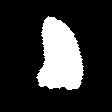
\includegraphics[width=0.5\textwidth]{binaryMask.jpg}
  \caption{Mask obtained from the collected boundary points.}
  \label{fig:second}
\end{figure}
 
As final step, we addressed mask storage. At this instance, we stored the generated masks as image files, each uniquely identified by a filename indicating the frame number and the corresponding video. This nomenclature facilitates easy identification for subsequent processing and analysis.


\subsection{Data Augmentation}
Data augmentation is a technique for artificially increase the size of a dataset by applying various transformations to the existing data \cite{augmentation}. For this process our primary goal is to enhance the diversity and variability of the training set. 

Firstly, we applied three distinct transformations to enhance the diversity of our dataset. These transformations included a 20° rotation, a 0.2 zoom, and a horizontal flip. Each original image contributed to the creation of three additional augmented images, resulting in a total of four versions, original and three augmented, for every input image, as illustrated in Fig. \ref{fig:DataAug}.

 \begin{figure}[H]
  \centering
  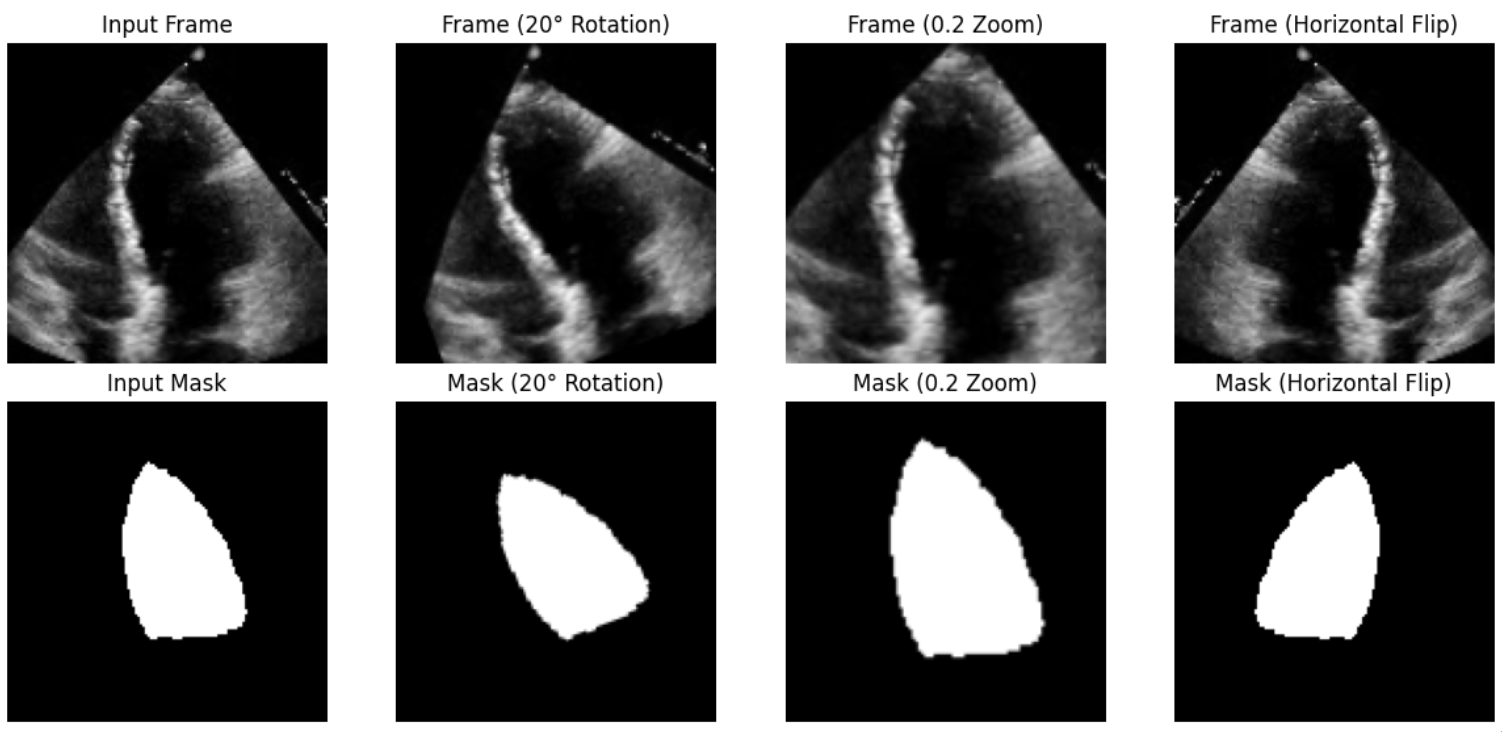
\includegraphics[width=0.9\textwidth]{DataAug.jpg}
  \caption{Data Augmentation.}
  \label{fig:DataAug}
\end{figure}

Out of the initial pool of 3,000 images, 80\% (2,400 images) were allocated for training purposes. Notably, the data augmentation techniques were selectively applied to two-thirds of the training set, encompassing 1,600 images. Consequently, post-augmentation, the training dataset expanded to a substantial 7,200 images, that is 1,600 augmented images $\times$
 4 transformations $+$ 800 non-augmented images.
 
This augmented dataset comprised a total of 7,200 frames, each paired with its corresponding mask. The augmentation process significantly contributed to the richness and variability of the training data, thereby enhancing the robustness and generalization capabilities of our neural network model. 

The shape of the augmented training images is (7200, 128, 128, 1), indicating a total of 7200 images with dimensions of 128 pixels by 128 pixels and a single channel. Similarly, the shape of the augmented training masks is (7200, 128, 128, 1), denoting 7200 masks with the same dimensions.

\subsection{Dataset division: Train-Validation-Test}
A total of 3200 images were sourced from the video frames of the echocardiogram dataset. Among these, 3000 images were processed, allocating 2400 for training purposes and 600 for validation. The remaining set of 200 images constituted the test dataset. However, the total number of training images fluctuated and increased due to the data augmentation step, where two-thirds of the images in this set were quadrupled, resulting in a final training set of 7200 images after accounting for the untouched third. Combining these with the 600 validation and 200 test images, we had a total of 8000 images, each paired with its corresponding mask.

\section{Model Architecture}
\subsection{U-net}
Neural networks, inspired by the intricate workings of the human brain, are computational systems comprised of interconnected units known as neurons. As described by Schmidhuber \cite{nn}, input neurons receive signals similar to how sensors perceive the environment, while other neurons activate through weighted connections from previously active neurons. This process often requires a series of computational stages where the network's collective activation is transformed, paving the way for the concept of deep learning, wherein credit is accurately allocated across multiple stages.

Convolution is a fundamental mathematical operation employed in signal processing and deep learning. In the context of neural networks, convolution involves the element-wise multiplication of a small matrix, called a kernel or filter, with a larger input matrix. This operation is pivotal for tasks like feature extraction, allowing the network to detect patterns and spatial hierarchies within the input data. Convolutional layers in neural networks utilize this operation to scan through input data and learn relevant features, facilitating the network's ability to recognize complex patterns \cite{b}.

Convolutional Neural Networks (CNN) represent a specialized class of neural networks designed for tasks involving grid-like data, such as images and videos. CNNs leverage convolutional layers to systematically apply filters to input data, capturing hierarchical features and spatial relationships. This architectural design makes CNNs particularly effective for image recognition, segmentation, and other computer vision tasks. The convolutional layers, in conjunction with pooling layers, enable CNNs to automatically and adaptively learn spatial hierarchies of features from the input data \cite{c}.

The U-net, a specialized architecture in deep learning, holds its name from its U-shaped design resembling the letter "U." This structure enables precise image segmentation, especially beneficial in fields like biomedical image processing. Unlike traditional convolutional networks, the U-net features a unique symmetric expansive path complementing the contracting path, enabling high-resolution outputs. Its architecture includes encoding layers for feature extraction and decoding layers for precise localization by upsampled outputs. Developed to address challenges in biomedical tasks, it excels in pixel-level class labeling, crucial for understanding complex images, such as those in medical diagnostics. By combining context information efficiently across different resolution layers, the U-net offers enhanced performance even with limited training data. Its distinctive design and adaptability make it a pivotal tool in various image segmentation tasks, providing accurate and detailed insights into intricate visual data such as ours, the echocardiograms \cite{unet}.
Below is an example of a visual representation of a U-net convolutional neural network architecture for medical image segmentation. Retrieved from: \url{https://lmb.informatik.uni-freiburg.de/people/ronneber/u-net/}.

\begin{figure}[H]
  \centering
  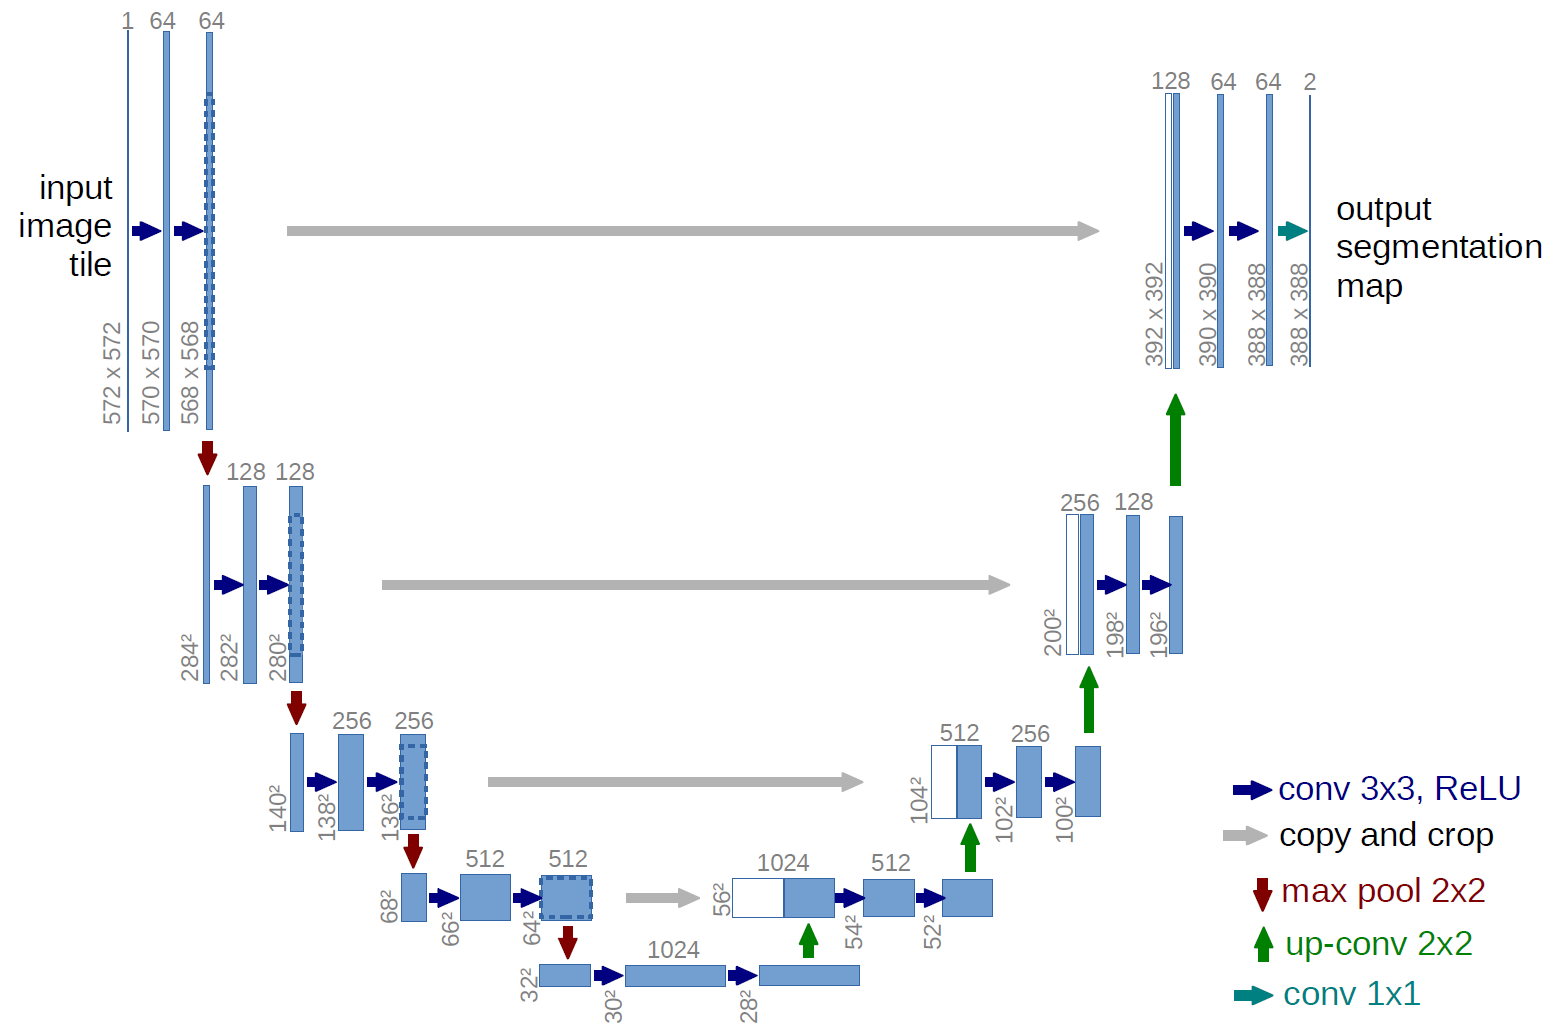
\includegraphics[width=0.5\textwidth]{u-net-architecture.png}
  \caption{U-net architecture.}
  \label{fig:unet}
\end{figure}

\section{U-net Methodologies}
\subsection{Masks}
Our first step in this methodology was started by loading and preprocessing images and corresponding masks. The code utilizes the OpenCV library to read, resize, and normalize images and masks. It ensures uniformity in image sizes and converts pixel values to a scale between 0 and 1. Then we defined our data splitting, as we explained before, the dataset was divided into training and validation sets, with 80\% of the data used for training and the remaining 20\% for validation. Additionally, a separate set of test images was created for evaluating the model's performance.

Further, we decide to apply data augmentation techniques. The code includes functions for rotating images, applying zoom, and horizontal flipping. These augmented images were then added to the training dataset.

At this point, we have everything we need to start the definition of our U-Net model, this model comprises an encoder-decoder structure with skip connections. The layers consist of convolutional and transposed convolutional operations, along with dropout layers to prevent overfitting. As we had this ready we can move on to the model training. We compiled and trained the U-Net model using the Adam optimizer and a custom loss function based on the Dice coefficient. The training history, including dice coefficients for both training and validation sets, was monitored and visualized.

The trained model was evaluated on a set of test images, and the segmentation results were compared against ground truth masks. By then, the Dice coefficient was calculated for each test case. For the visualization and model summary we used visualization tools to inspect the model's architecture and created visualizations of the training history, including dice coefficient trends over epochs.

Around the final steps, we include a section for video processing and GIF creation; the code includes functions to apply the trained model to video frames, generate segmentation masks, and combine the masks with original frames to create visually informative GIFs. These GIFs showcase the model's ability to segment the left ventricle in dynamic heart images.
Finally, for the results and analysis, the final part of the code analyzes the Dice scores, calculates average scores, and presents them through histograms, providing insights into the model's overall performance.

In the following Fig. \ref{fig:unet model} , the final architecture of the constructed neural network is depicted.
\begin{figure}[H]
  \centering
  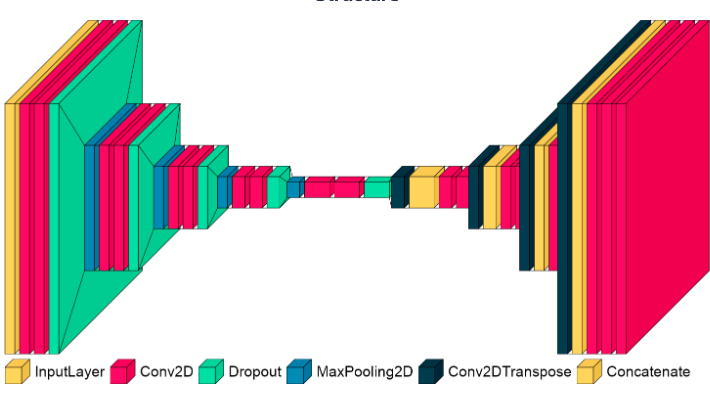
\includegraphics[width=0.5\textwidth]{unet.png}
  \caption{Final U-net architecture.}
  \label{fig:unet model}
\end{figure}

\subsection{Landmarks}
Landmarks are distinctive points or features in a given context that serve as reference points. In medical image segmentation, landmarks can be anatomical points or specific regions of interest within an image. When applying a U-Net for ventricular segmentation, landmarks could include crucial points within the heart anatomy, aiding the network in accurately delineating the boundaries of the ventricles.

In conjunction with landmarks, heatmaps emerge as a critical element, functioning as probability maps that express the likelihood of specific features across pixel locations within an image. These heatmaps are integral in indicating the probability associated with landmarks or boundaries within the cardiac anatomy. As the U-Net processes the images, it concurrently generates heatmaps assigning higher probabilities to pixels corresponding to significant landmarks or areas of interest within the heart. These probability cues guide the subsequent segmentation process, aiding the model in precisely delineating ventricular boundaries.

The symbiosis between landmarks and heatmaps is pivotal. Landmarks offer distinct reference points, and heatmaps augment this by assigning probabilities to their presence. This collaborative approach enhances the segmentation process, contributing to the model's precision in identifying and delineating the cardiac structure.

Having established a conceptual foundation on the pivotal roles of landmarks and heatmaps, we now delve into the practical application of this methodology within the U-Net architecture. The journey begins with a meticulous selection of landmarks for ventricular segmentation, involving a systematic process aimed at identifying anatomically significant points. Specifically, a function was employed to choose six landmarks. The first two were determined by selecting the topmost and bottommost points based on their Y-coordinates. Subsequently, these points were divided into 80\% and 20\% split, as shown in Fig. \ref{fig:sol}.

\begin{figure}[H]
    \centering
    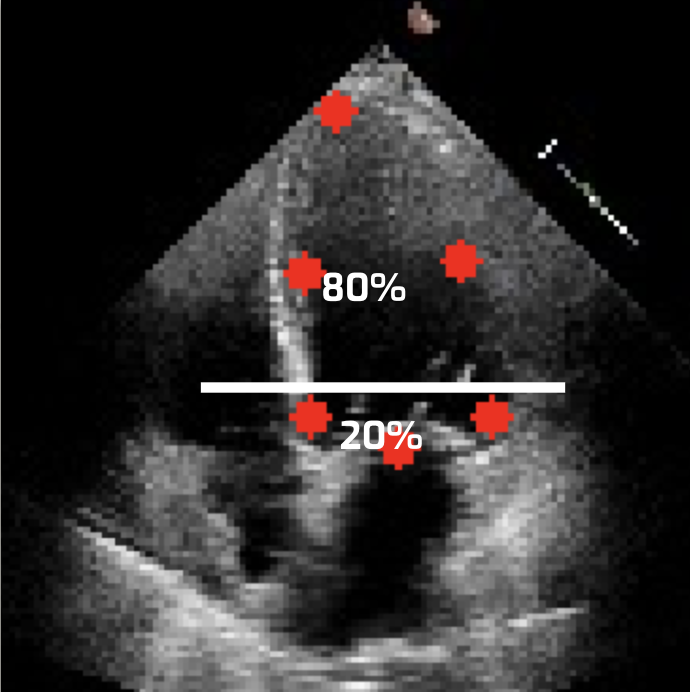
\includegraphics[width=0.5\textwidth]{sol.jpg}
    \caption{Landmark Selection Process}
    \label{fig:sol}
\end{figure}

Within the 20\% subset, the points with the furthest left and right positions were chosen, creating a spatially diverse representation. The final two landmarks were determined by calculating the curvature of each point concerning its preceding and succeeding points, ensuring a nuanced selection based on the ventricular anatomy's curvature characteristics. 

The curvature calculation provided a quantitative measure of the anatomical features, ensuring that the chosen landmarks encapsulated critical aspects of the ventricular structure. This selection aimed to capture both spatial and curvature diversity within the chosen landmarks.

Once the six landmarks were established, individual heatmaps were generated for each landmark. These heatmaps served as the inputs to the segmentation model, resulting in six distinct images, each highlighting a specific region of interest within the ventricle, as illustrated in Fig. \ref{fig:hm}. As mentioned before, the heatmaps, functioning as probability maps, conveyed the likelihood of significant features at various pixel locations.

\begin{figure}[H]
    \centering
    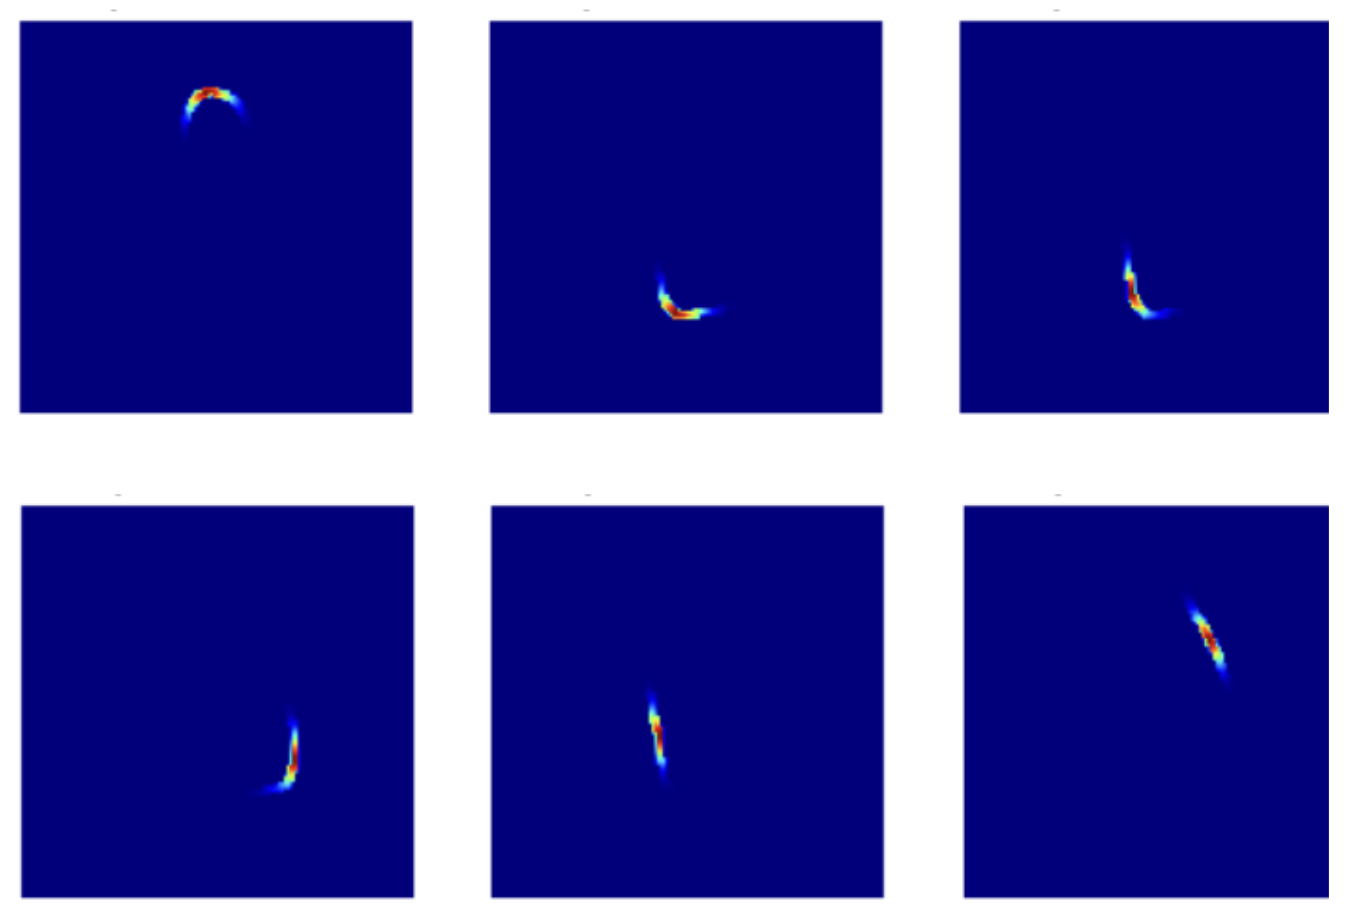
\includegraphics[width=0.7\textwidth]{hm.jpg}
    \caption{Individual Heatmaps}
    \label{fig:hm}
\end{figure}

In terms of layer complexity, the model embraced a range of convolutional layers employing a varied filter count, spanning from 64 to 1024.

After obtaining the heatmaps, the dataset underwent a division process. Similar to the previous mask method, the initial pool consisted of 7000 images, each accompanied by its respective 7000 heatmaps. This dataset division allocated the following subsets for both images and heatmaps: 4200 for training and 2800 for validation, with a further breakdown within the validation subset resulting in 2601 for validation and 199 for testing. Post augmentation in the training set involving a 20° rotation, 0.2 zoom, and 
a horizontal flip, the dataset grew to encompass a total of 8268 images, each matched with its corresponding heatmaps. The final dimensions settled at (8268, 112, 112, 3) for images and (8268, 112, 112, 6) for heatmaps. These dimensions signify the number of images, pixel dimensions, and channels—3 for images (representing the rgb: red, green, and blue) and 6 for heatmaps, indicating six heatmaps per image.

The modified U-Net model adapted for generating six heatmaps per image. This model architecture consists of an encoder-decoder network structure, adept at processing and understanding complex image features. The encoder portion involves a sequence of convolutional layers followed by pooling operations, effectively capturing hierarchical representations of the input images. Subsequently, the bottleneck section condenses and extracts crucial information from these representations. The decoder phase reverses the process, upscaling the condensed information back to the original image dimensions. By using transposed convolutional layers and concatenating feature maps at each step, this architecture aims to recover spatial information lost during the encoding stage. Finally, the model outputs six channels, representing the six generated heatmaps for each input image. The model is trained using the Adam optimizer and binary cross-entropy loss function, aiming to minimize the difference between predicted and ground truth heatmaps. Additionally, the model's performance is evaluated using the Dice coefficient metric, measuring the agreement between predicted and true segmentation masks. 

\subsubsection{Post-processing}
The model underwent training for 30 epochs, following which we conducted result visualization by superimposing the generated heatmaps onto a random image. Additionally, we extracted landmarks from these heatmaps, sorting them based on their positions, and subsequently generated masks utilizing OpenCV and scipy interpolation techniques. In the visual representation presented in the Fig. \ref{fig:output}, multiple output examples are showcased.

\begin{figure}[H]
    \centering
    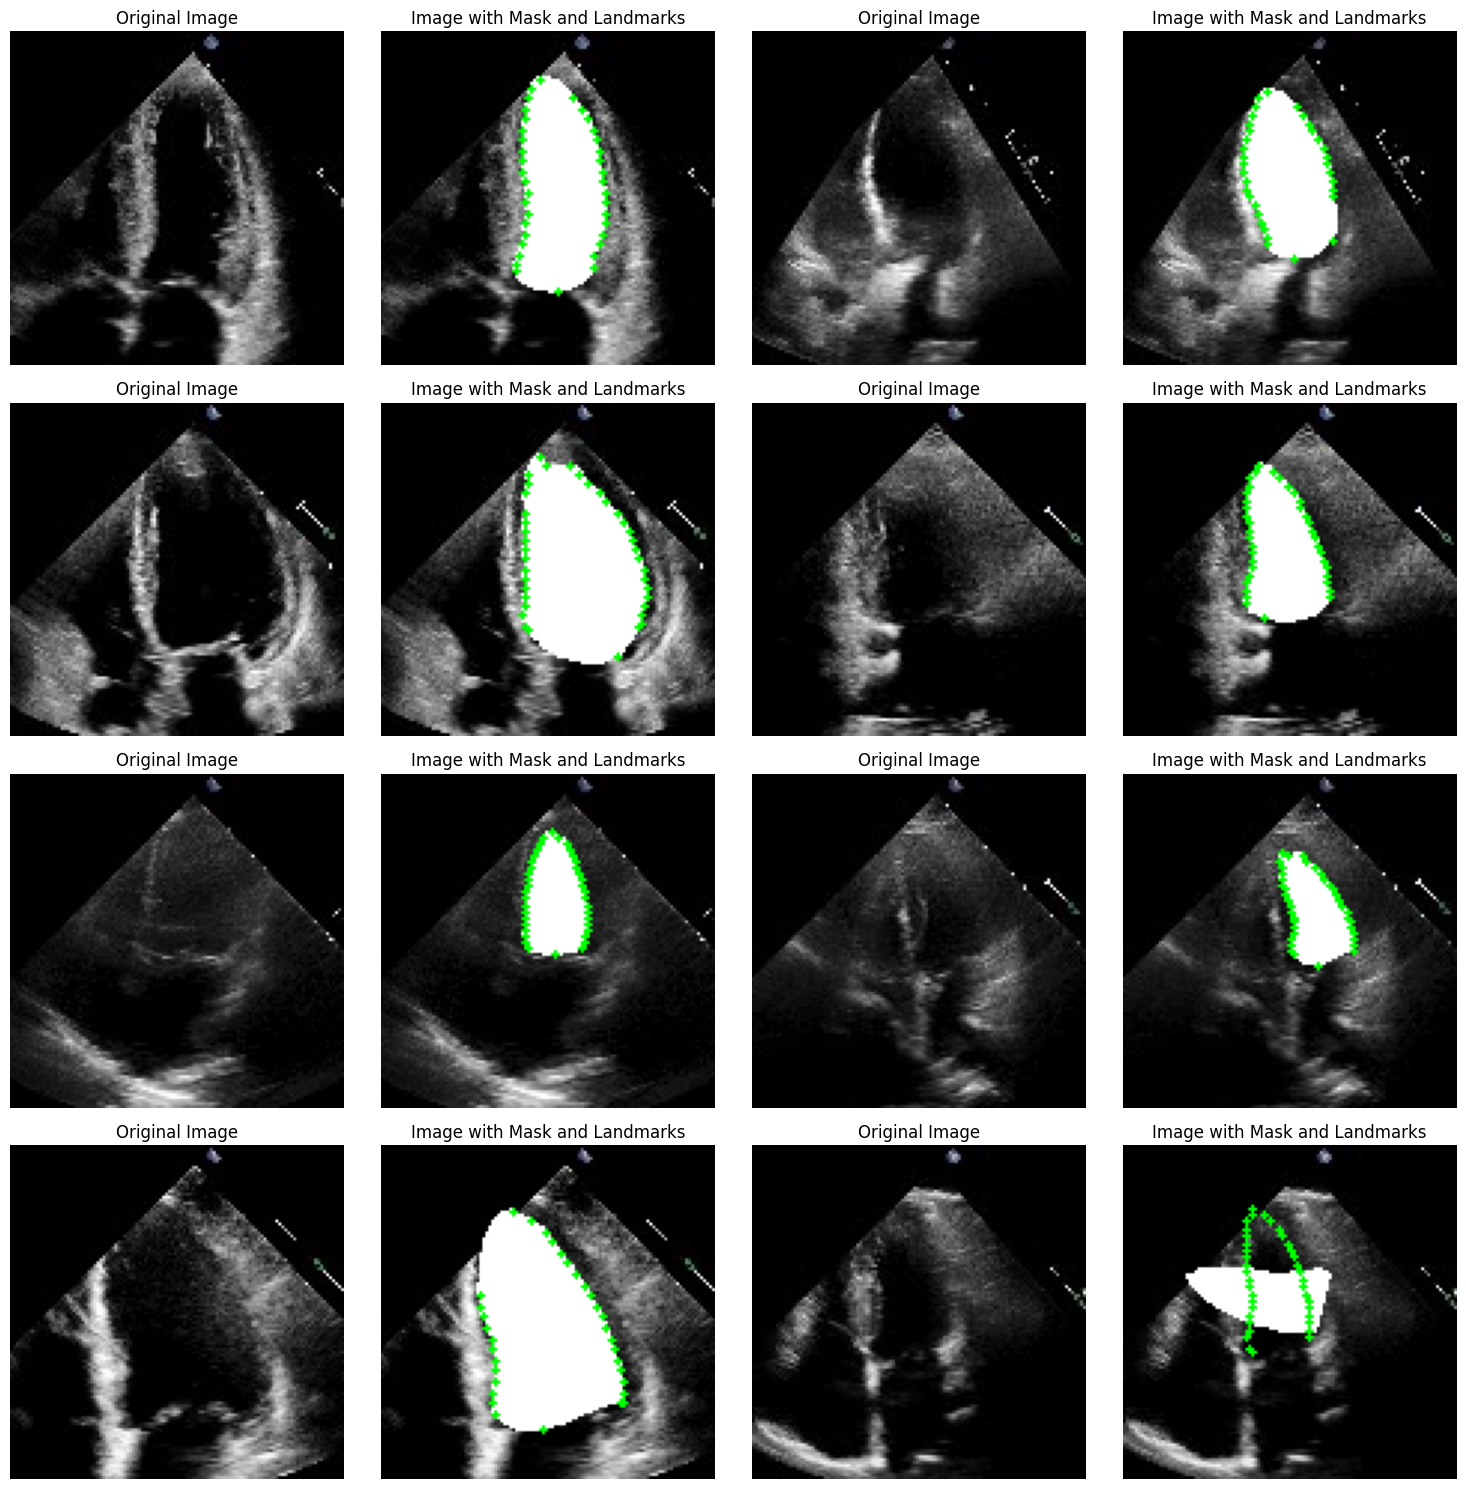
\includegraphics[width=0.7\textwidth]{output.png}
    \caption{U-net landamarks mask output}
    \label{fig:output}
\end{figure}
An observation to note is occasional misalignment in the mask's positioning. This discrepancy arises due to inaccuracies in the spline interpolation process, which unexpectedly receives erroneous inputs. Despite this, it's worth noting the consistent accuracy in landmark display, contrasting the occasional misplacement in the generated mask. Identifying the specific cause behind this discrepancy remains an ongoing challenge within our research efforts.

Similar to the previously outlined methodology, the efficacy of the trained model was assessed across a test image set and an external dataset, with the resultant segmentation outputs compared against ground truth masks. This comparison was quantified using the Dice coefficient, calculated for each test case to gauge the model's accuracy. In the latter stages, a specialized section dedicated to video processing and GIF creation was incorporated into the codebase. This section encompasses functionalities facilitating the application of the trained model to video frames, the generation of segmentation landmark-based masks, and the synthesis of these masks with original frames to craft informative GIFs. Subsequently, in the results and analysis phase, the concluding segment of the code systematically analyzes the Dice scores, computes average scores, and presents them visually through histograms. This graphical representation offers comprehensive insights into the overall performance of the modified U-net model, aiding in the discernment of its efficacy and limitations.


\subsection{Dice Score}
The Dice Score is a metric commonly used to evaluate the performance of segmentation algorithms, including those based on neural networks. It quantifies the similarity between the predicted segmentation mask and the ground truth mask by measuring the overlap between them \cite{dice}.

The formula for the dice score is given by:

\begin{equation}
DiceScore = \frac{2 \cdot \left | Intersection \right |}{\left | Predicted \right |+\left | GroundTruth \right |}
\end{equation}
Where:
\begin{itemize}
    \item Intersection: Represents the number of pixels that are both in the predicted mask and the ground truth mask.
    \item Predicted: Is the total number of pixels in the predicted mask.
    \item Ground Truth: Is the total number of pixels in the ground truth mask.
\end{itemize}

The Dice Score ranges from 0 to 1, with 1 indicating a perfect overlap between the predicted and ground truth masks. A higher Dice Score signifies better segmentation performance, reflecting the accuracy and precision of the segmentation algorithm in capturing the true positive pixels while minimizing false positives and false negatives \cite{dice}.

\subsection{Models Comparison}

\subsubsection{Masks Model Segmentation Results}
The U-Net model trained with binary masks demonstrates a robust performance on the validation set, achieving a Model (validation) Dice Score of 91.56\%. Examining the epoch-based training dynamics, the training Dice Score steadily ascends, reaching a stabilization point around epoch 12.5, thereafter exhibiting gradual improvement. Concurrently, the validation Dice Score maintains stability, fluctuating between 0.90 and 0.91, indicating a consistent and accurate segmentation performance, as shown in Fig. \ref{fig:m1}.

\begin{figure}[H]
    \centering
    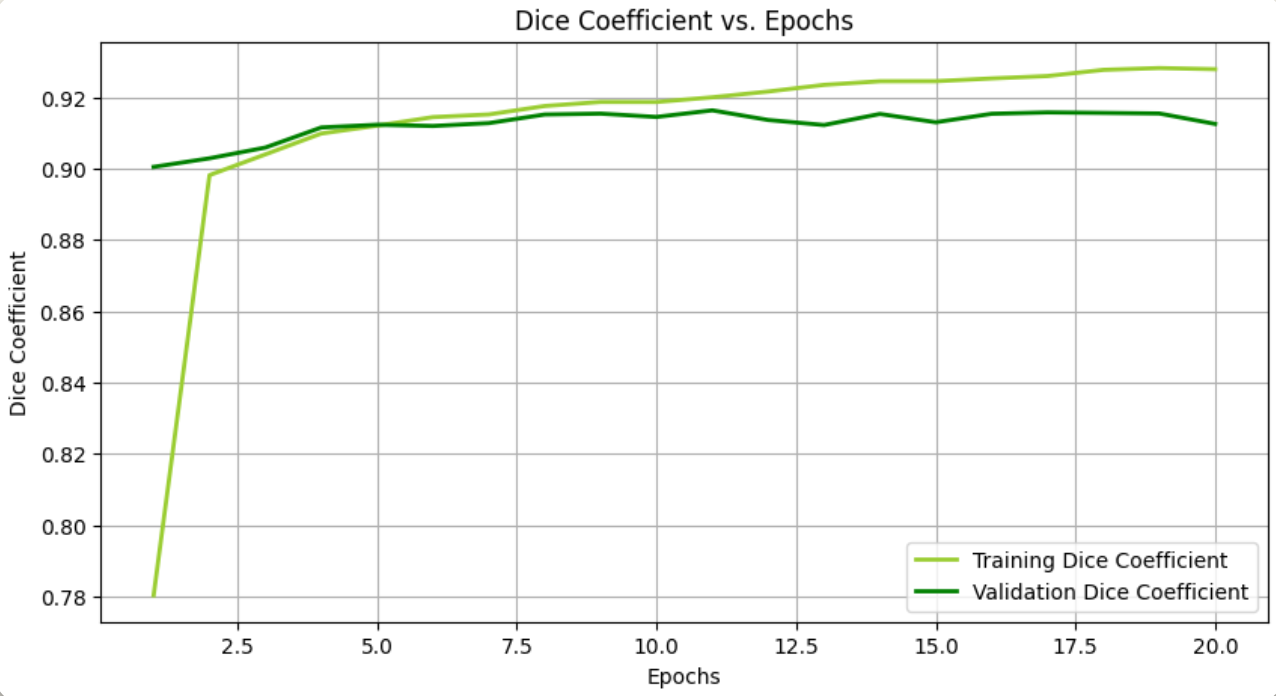
\includegraphics[width=1.0\textwidth]{m1.jpg}
    \caption{Performance on the validation set}
    \label{fig:m1}
\end{figure}

The segmentation results, as illustrated in Figure \ref{fig:m1s}, visually confirm the model's proficiency in delineating the left ventricle in the echocardiogram images.

\begin{figure}[H]
    \centering
    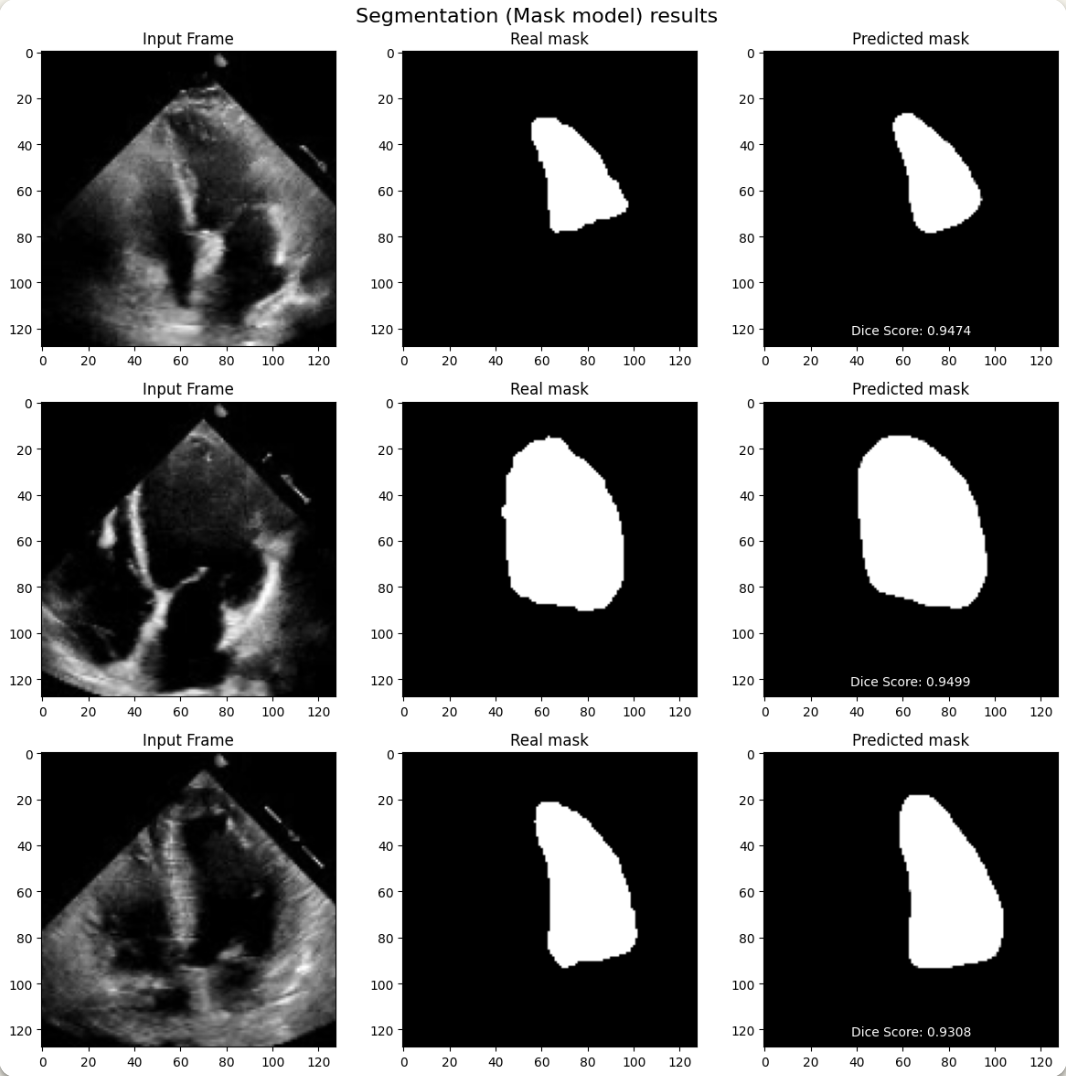
\includegraphics[width=1.0\textwidth]{m1s.jpg}
    \caption{Segmentation results on validation set}
    \label{fig:m1s}
\end{figure}

The Mean Dice Score on the test set for binary masks is reported at 91.58\%. The accompanying graph depicting the Dice Score distribution, as presented in Figure \ref{fig:histogramam}, reveals not only the overall high mean but also instances of exceptional segmentation accuracy exceeding 0.95\%. The segmentation visualizations, showcased in Figure \ref{fig:ms}, further validate the model's capability, illustrating the predicted masks overlaid on the original echocardiogram images.

\begin{figure}[H]
    \centering
    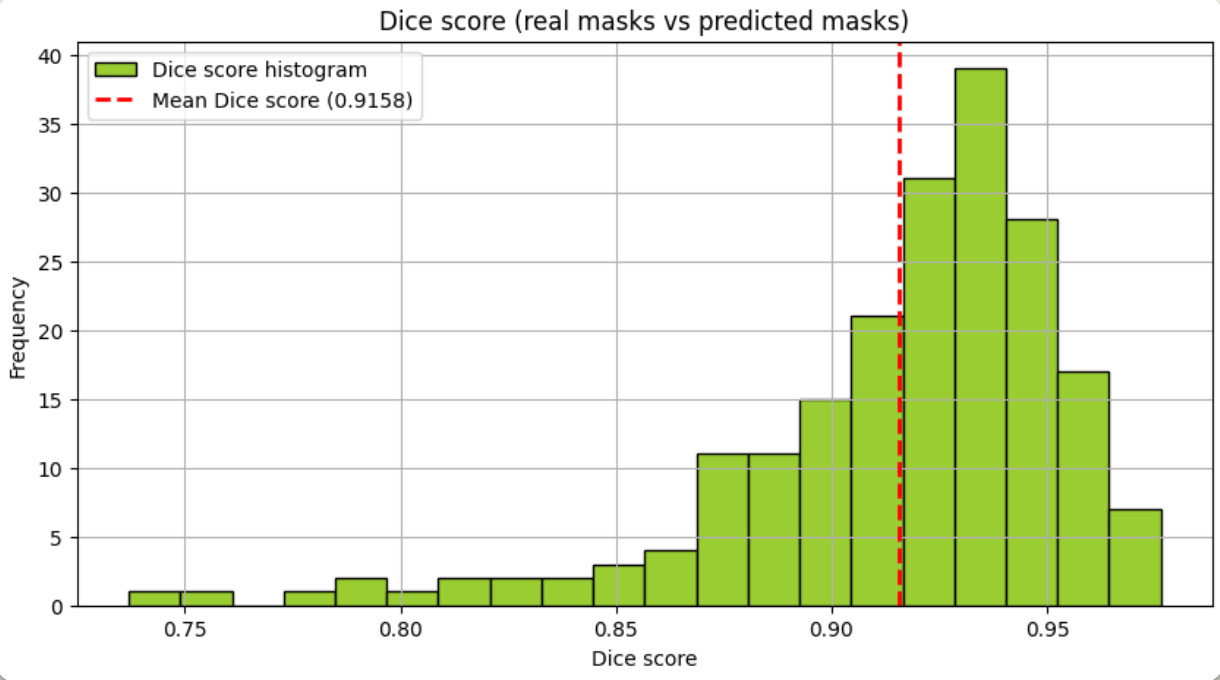
\includegraphics[width=1.0\textwidth]{histogramam.jpg}
    \caption{Performance results on test set}
    \label{fig:histogramam}
\end{figure}

\begin{figure}[H]
    \centering
    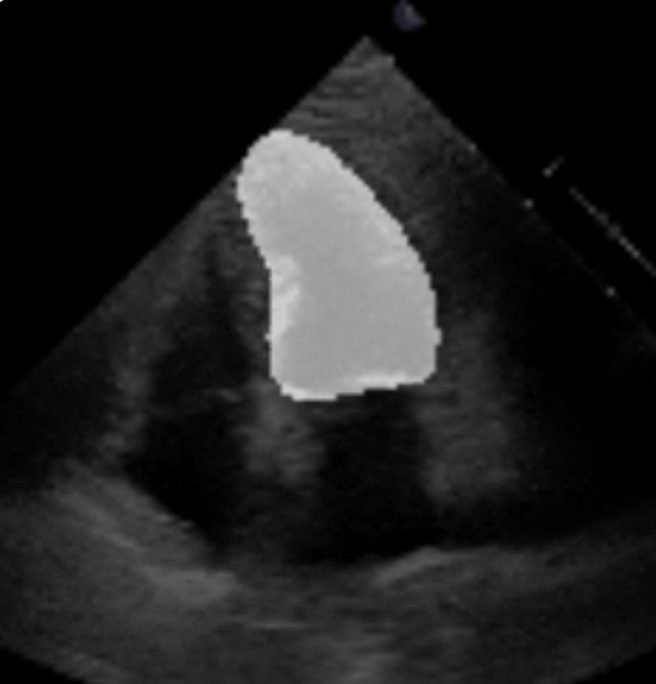
\includegraphics[width=0.5\textwidth]{ms.jpg}
    \caption{Segmentation results on test set}
    \label{fig:ms}
\end{figure}

\subsubsection{Landmarks Model Segmentation Results}

In the landmark-based approach, the Mean Dice Score on the test set is reported at 91.14\%. Figure \ref{fig:histogramalm} provides a frequency distribution of Dice Scores, offering insights into the segmentation performance variability. Despite the slightly lower mean, examination of the distribution reveals instances where the model achieved Dice Scores slightly surpassing the mean. The segmentation visualizations, presented in Figure \ref{fig:lm1s}, offer a qualitative assessment, demonstrating the predicted masks superimposed on the original echocardiogram images.

\begin{figure}[H]
    \centering
    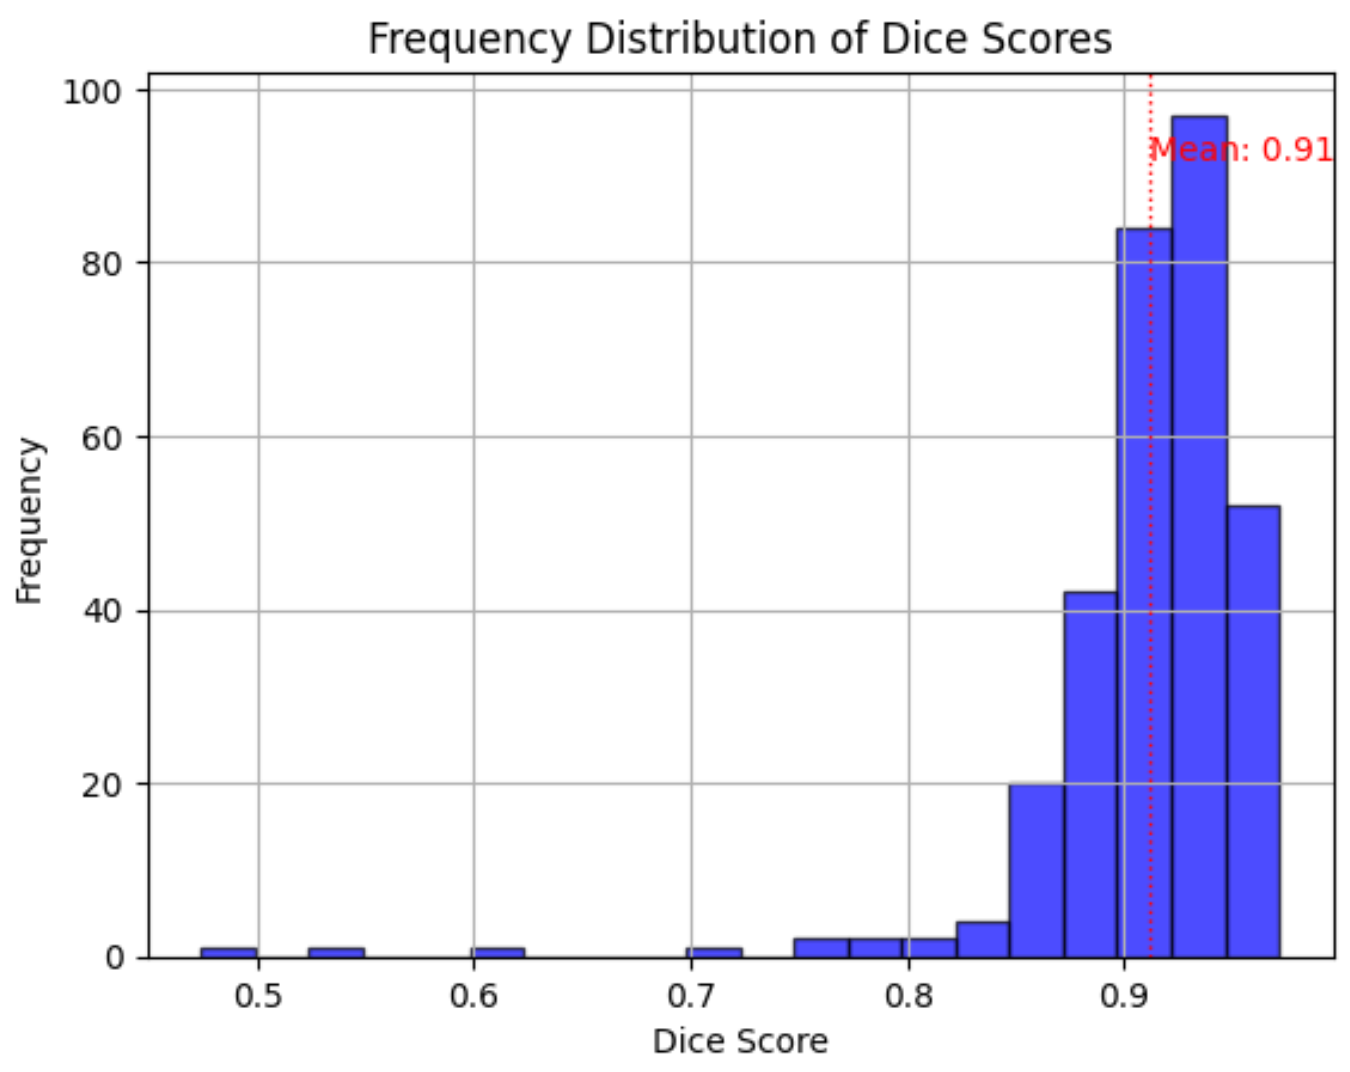
\includegraphics[width=0.7\textwidth]{histogramalm.jpg}
    \caption{Performance results on Landmarks Model}
    \label{fig:histogramalm}
\end{figure}

\begin{figure}[H]
    \centering
    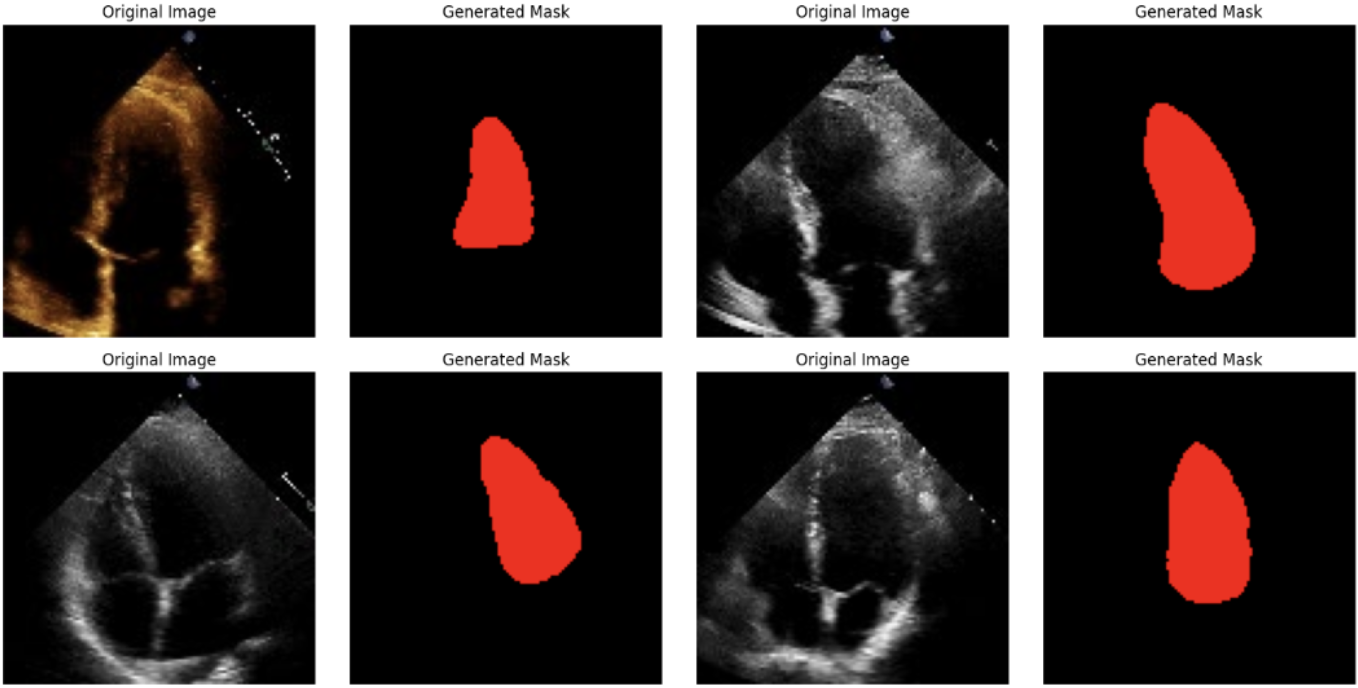
\includegraphics[width=0.7\textwidth]{lm1s.jpg}
    \caption{Segmentation results on Landmarks Model}
    \label{fig:lm1s}
\end{figure}

\section{Experimental setup}
\subsection{Github}
The following link directs to our GitHub repository housing all the codes developed for this research, along with other pertinent information in the field. Explore the repository and related resources here: 

\url{https://github.com/IA-Avanzada/Reto2}

\subsection{Hardware}
While the dataset description does not provide specific hardware details, it is essential to understand the typical equipment required for acquiring echocardiogram videos:

\begin{itemize}
    \item[$\bullet$] \textbf{Ultrasound machine}: The primary device for performing echocardiograms. It is equipped with probes or transducers that emit ultrasound waves and capture reflected signals to generate real-time images of the heart.
    \item[$\bullet$] \textbf{Monitor}: To visualize the real-time images during the procedure. 
    \item[$\bullet$] \textbf{Transducer}: A device that emits and receives high-frequency sound waves (ultrasound) to create images of the heart. The type and frequency of the probe vary depending on the specific imaging needs, such as the apical-4-chamber probe used in the dataset.
    \item[$\bullet$] \textbf{Video Recording Equipment}: To capture and save the videos produced during the procedure.
    \item[$\bullet$] \textbf{Computer and Software}: Essential for data processing, storage, and report generation. Specialized software may be used for image analysis.
    \item[$\bullet$] \textbf{Examination Bed}: A bed or surface where the patient is positioned for the echocardiogram.
\end{itemize}

\subsection{Software}
The software used, specifically using the U-Net architecture, involves a combination of Python, Jupyter Notebook, and several essential libraries. The following outlines the key components of the software environment:

\begin{itemize}
    \item[$\bullet$] \textbf{Python}:  The program is designed to be compatible with Python 3.x, and it is recommended to have Python installed on the system.
    \item[$\bullet$] \textbf{Jupyter Notebook environment}: The program assumes access to a Jupyter Notebook environment, either locally installed or web-based, for code execution and visualization.
    \item[$\bullet$] \textbf{Utilized libraries}:
        \begin{itemize}
            \item[$\bullet$] \textbf{Pandas}: For manipulating data using DataFrames.
            \item[$\bullet$] \textbf{Numpy}: Numerical operations and array manipulations.
            \item[$\bullet$] \textbf{Scikit-learn}: For machine learning tasks, such as train-test splitting.
            \item[$\bullet$] \textbf{TensorFlow}: For deep learning tasks, and in this case, for building and training neural networks.
            \item[$\bullet$] \textbf{Keras}: Integrated with TensorFlow, is used for defining the neural network architecture.
            \item[$\bullet$] \textbf{Matplotlib}: For creating visualizations, such as plotting graphs.
            \item[$\bullet$] \textbf{Imageio}: Enables reading and writing of images and videos.
            \item[$\bullet$] \textbf{Scipy and Skimage}: Used with the ndimage module, dor image processing tasks.
        \end{itemize}
    \item[$\bullet$] \textbf{Dataset}: The program relies on the EchoNet-Dynamic dataset for cardiac image segmentation.
\end{itemize}


\section{Conclusions}
In conclusion, while the model utilizing masks exhibited a higher Dice score, the landmark-based model demonstrated superior practical performance. This distinction arises from the landmark model's potential utility in real-world applications, particularly in a medical context. Its advantage lies in the ease of correction; in a prospective deployment scenario, end-users could effortlessly refine predicted masks by simply adjusting landmark positions. This attribute holds significant promise for practical implementation, as it offers an intuitive and user-friendly approach in medical image segmentation tasks. Moreover, these findings underscore the significant strides made in leveraging deep learning and image segmentation within the medical domain. The use of sophisticated algorithms not only showcases remarkable accuracy in delineating and analyzing medical imagery but also holds immense potential in revolutionizing diagnostic and treatment methodologies. The integration of deep learning models in medical image segmentation heralds a promising era, where precision, efficiency, and user-friendliness converge to augment and refine medical practices, potentially improving patient care and diagnostic accuracy in the foreseeable future.


\newpage
\section{Individual Contributions}
\begin{enumerate}
    \item \textbf{Alfonso Pineda} \\
    
    Alfonso Pineda played a significant role in the development of the mask model, taking charge of the final version and consistently updating it to achieve optimal performance and results. His contributions extended beyond the model development, as he conducted a comprehensive analysis and comparison of the obtained results by evaluating the model with both the initial dataset and an external dataset.\\

    In the preprocessing phase of the landmark model, Alfonso was actively involved in creating all the contours used for training, Gaussian heatmaps, and their corresponding probability maps. This meticulous work significantly contributed to the quality of the landmark model.\\
    
    Moreover, Alfonso contributed to the preprocessing of the mask model, refining the final landmark sorting method for the generation of training masks and dataset splitting. His multifaceted involvement ensured the efficiency and coherence of the entire project.\\
    
    Additionally, Alfonso played an integral role in the collaborative effort to compose this research report, providing valuable insights and contributing to the overall coherence of the document. \\
    
    \item \textbf{Álvaro Morán} \\
    
    Álvaro Morán played a crucial role in the project, particularly in the development of the final Landmarks model. He led the creation of the final version of the model, implementing consistent updates to optimize its performance and results. Similar to his counterparts, Álvaro conducted a meticulous evaluation of the model's results using both the initial dataset and an external dataset, providing valuable insights through a comprehensive analysis and comparison.\\

    Additionally, Álvaro was involved in the creation of a secondary landmarks model based on coordinates, although this model remained inconclusive. His contributions in exploring alternative approaches demonstrated a commitment to thorough exploration and experimentation within the project.\\
    
    Furthermore, Álvaro actively contributed to the preprocessing phase of the landmark model by creating an algorithm to identify the six ideal landmarks for each frame. This preprocessing step significantly impacted the quality of landmark data used in the model.\\
    
    In conjunction with his technical contributions, Álvaro played an active role in the collaborative effort to compose this research report, ensuring that his insights were seamlessly integrated into the overall narrative.\\
    
    \item \textbf{Mariana Rincón}\\
    
    Mariana Rincón made notable contributions to the project, particularly in the development of the function responsible for extracting frames based on the 'VolumeTracings.csv' file, its corresponding records, and the videos contained in the 'EchoNet-Dynamic' dataset. Her involvement in this aspect ensured a systematic and accurate extraction of frames for subsequent analysis.\\
    
    Additionally, Mariana played a crucial role in the preprocessing phase of the mask model, where she successfully generated masks for the frames mentioned earlier. Moreover, Mariana actively participated in the collaborative effort to compose this research report, providing valuable insights and contributing to the overall coherence of the document.\\
    
    \item \textbf{Karla González}\\
    Karla González played a crucial role in the project, particularly in the realm of data augmentation. She actively contributed to the creation of functions for data augmentation in both training datasets for the models.\\
    
    Furthermore, Karla took charge of generating graphical representations that effectively illustrated the processes and functionalities of the functions developed. These graphics served a dual purpose, enriching both the content of the research report and the final presentation.\\

    In addition to her technical contributions, Karla actively participated in the collaborative effort to compose this research report, ensuring that her insights were integrated cohesively into the overall narrative.\\
    
    \item \textbf{Salvador Mendoza}\\
    
    Salvador Mendoza played a pivotal role in the initial stages of the mask model's creation, offering insightful proposals for architectures that significantly influenced the development of the final version. His contributions during this crucial phase provided a foundation for the subsequent refinement of the model.\\

    Additionally, Salvador actively participated in generating graphical representations that effectively illustrated the processes and functionalities of various functions within the project. These graphics not only enhanced the visual appeal of the research report but also served as valuable tools for communicating the intricacies of the developed methodologies.\\
    
    Furthermore, Salvador was an integral part of the collaborative effort to compose this research report, contributing his expertise and insights to ensure a comprehensive and well-documented account of the project.
\end{enumerate}

\newpage
\printbibliography
\end{document}

